\documentclass[usenames,dvipsnames]{beamer}
    \mode<presentation> {
    \usetheme{Montpellier}
    \usecolortheme{beaver}
    %\setbeamertemplate{footline} % To remove the footer line in all slides uncomment this line
    \setbeamertemplate{footline}[page number] % To replace the footer line in all slides with a simple slide count uncomment this line

    \setbeamertemplate{navigation symbols}{} % To remove the navigation symbols from the bottom of all slides uncomment this line
    }

    \usepackage{graphicx} % Allows including images
    \usepackage{booktabs} % Allows the use of \toprule, \midrule and \bottomrule in tables
    \usepackage{minted}
    \usepackage{xcolor}
    %\usepackage[mathletters]{ucs}
    %\usepackage[utf8x]{inputenc}
    \usepackage[utf8]{inputenc}
    \usepackage{pifont}    
    \usepackage{newunicodechar}
    \newunicodechar{✪}{\ding{74}}

    %\DeclareUnicodeCharacter{272A}{\star}
    \definecolor{mintedbackground}{rgb}{0.95,0.95,0.95}
    \newcommand{\code}[1]{\colorbox{lightgray}{\texttt{#1}}}


\newmintedfile[scalacode]{scala}{
bgcolor=mintedbackground,
fontfamily=tt,
linenos=true,
numberblanklines=true,
numbersep=5pt,
gobble=0,
frame=leftline,
framerule=0.4pt,
framesep=2mm,
funcnamehighlighting=true,
tabsize=4,
obeytabs=false,
mathescape=false
samepage=false, %with this setting you can force the list to appear on the same page
showspaces=false,
showtabs =false,
texcl=false,
}
    \setminted{fontsize=\footnotesize,baselinestretch=1}

    \usepackage {tikz}
    \usetikzlibrary {positioning}
    \graphicspath {{target/media/}}
    %----------------------------------------------------------------------------------------
    %	TITLE PAGE
    %----------------------------------------------------------------------------------------

    \title[Roles]{Roles: a viable alternative to Microservices and Monoliths}

    \institute[Septimal Mind Ltd]
    {
    Septimal Mind Ltd\\
    \medskip
    \textit{team@7mind.io}
    }
    \date{\today}

\begin{document}

\begin{VerbatimOut}{ex-scala-roles.tmp}
@RoleId("testservice") 
class TestService[F[_] : Monad](http: HttpSrv[F]) 
  extends IzService {
    override def start(): Unit = http.start()
    override def stop(): Unit = http.stop()
}
class TestPlugin extends PluginDef {
  many[IzService].add[TestService[IO]]
}
object TestLauncher {
  // you may run it like `test.jar test-service other-service`
  def main(args: Array[String]): Unit = IzRoleApp(args).main()
}
\end{VerbatimOut}

\begin{frame}
\titlepage
\end{frame}

\section{The problem: both Monolith and Microservice approaches are broken}

\begin{frame}
\frametitle{Monoliths are broken}
We all know that Monoliths aren't nice:
\begin{itemize}
\item Provoke tight-coupling and non-SOLID code,
\item When you deploy you need to deploy everything (not always a bad thing),
\item Startup time is usually high,
\item Inconvenient when your codebase is large: you may need to rebuild to much, etc,
\item Dependency convergence.
\end{itemize}

Structuring, conventions and different enforceable boundaries may mitigate some issues.

Pulling conservative parts out of the main codebase into independent libraries helps.
\end{frame}

\begin{frame}
\frametitle{We have Microservices}
Microservices are intended to address Monolithic Design problems.
\begin{itemize}
\item They put strict isolation on software components,
\item Convergence issues are addressed by isolation as well,
\item They simplify scaling (in case you ``Design Properly''),
\item You may redeploy independent components,
\item \dots
\end{itemize}
\begin{figure}
    \Large BUT\dots
\end{figure}
\end{frame}

\begin{frame}
\frametitle{You've seen this before}
\begin{figure}
    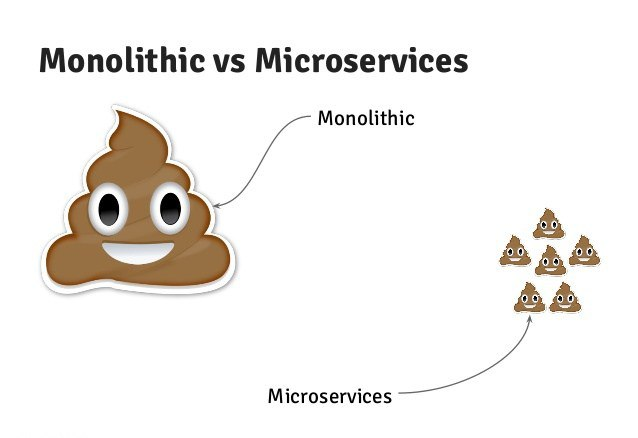
\includegraphics[width=0.9\textwidth]{media/mono-ms-joke.jpg}
\end{figure}
\end{frame}

\begin{frame}
\frametitle{The alternative -- Microservices -- is just sick}

\begin{itemize}
\item Evil Dependencies and neccessary \textit{Shared State},
\item Deployment and maintenance becomes more complicated with each new dependency,
\item Inevitably Distributed: all \textit{fundamental} problems are in place. CAP theorem?,
\item Cascading failures,
\item Accidental Incompatibilities: you may notice them too late. Amplified by cascade failures,
\item Computing Density: 50 JVM microservices in Docker on a single machine? Really?,
\item Overcomplicated Development Flows: a simple [integration\footnotemark[1]] test requires many things done in right order,
\item Time, interference and reproducible builds: isolated environments are expensive to setup.
\end{itemize}
\footnotetext[1]{Not a constructive definition. Subject of another presentation}
\end{frame}

\begin{frame}
\frametitle{Observations on Microservices}
\begin{itemize}
\item \textit{Software components} are still in place -- in form of Services.
      All the potential pitfails of component design apply to microservices,
\item Many checks which may be done by your compiler in case of monolithic design have  
     to be performed by integration test suites (in case you have them, it's hard to write),   
\item Many tasks are delegated to operations: in case of a monolith your dependency graph is being 
      processed by your DI framework\footnotemark[1], in case of microservices it is\dots in worst case processed by people,
      in best case requires an orchestration tool. But we don't have any single great tool yet,
\item An orchestration tool does \textit{exactly the same job} your DI framework may do. And lot more things.
\end{itemize}
\footnotetext[1]{Or an alternative mechanism with the same purpose}
\end{frame}

\section{The solution: roles}

\begin{frame}
\frametitle{Roles: the idea to rescue}
We need something with all the positive traits of Microservices and Monoliths but less negative.
\vspace{0.3cm}
\begin{itemize}
\item Let's run multiple services\dots in one service. Well, one process,
\item Let's choose which \textit{roles} we wish to assign to a before we start it,
\item Roles come from Classpath, may be discovered dynamically or statically,
\item It resembles Containers and OSGi,
\item Containers have some disadvantages. 
      They provide you a lot so we get used to think that they are sluggish on startup.
      Isolated classloaders are inconvenient. Dynamic DI is a nightmare,
\item Let's get rid of Dynamic DI. And let's keep isolation optional.
\end{itemize}
\end{frame}

\begin{frame}
\frametitle{Multi-Tenant Processes and Roles}
\begin{figure}
    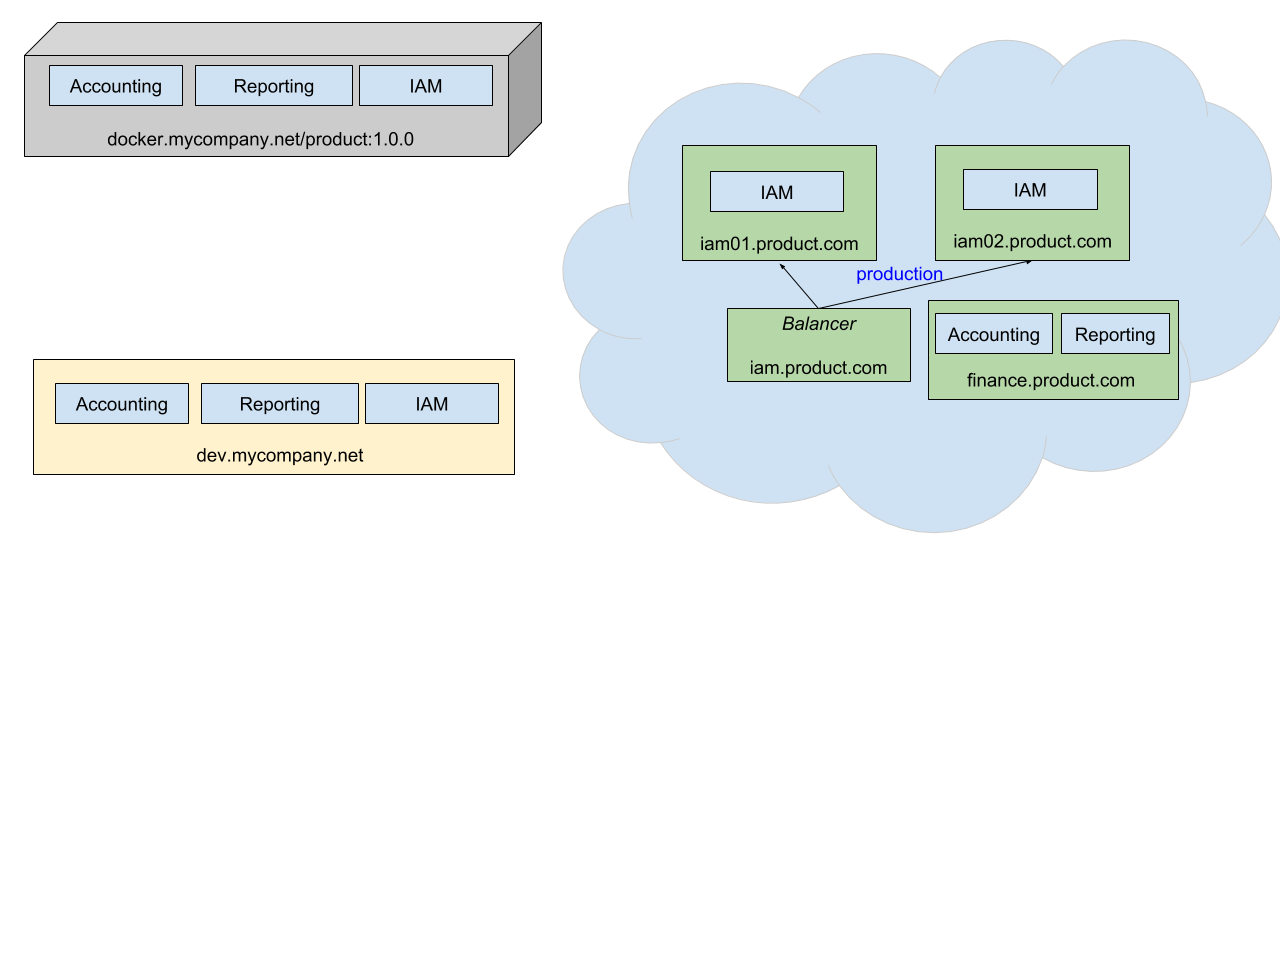
\includegraphics[width=\textwidth]{media/role-based-layout.png}
\end{figure}
\end{frame}

\begin{frame}
\frametitle{Benefits}
Roles allow you to do \textbf{everything} you can do with microservices plus have additional benefits\footnotemark[1]:
\begin{itemize}
\item Higher Density makes Development Flows better: instant startup of any combination of roles,
\item Higher Density makes Operations easier: any combination of roles for any container. 
    You don't need to start 5 containers to have 5 services with low load profile,
\item Smaller distribution size: Just one image, less traffic,
\item More static checks $\Rightarrow$ higher reliability,
\item Easier to setup environments (just run a process) $\Rightarrow$ easier to perform integration testing $\Rightarrow$ higher reliability, quicker delivery,
\item Quicker builds.
\end{itemize}
\footnotetext[1]{Roles do not solve \textit{all} the issues automagically}
\end{frame}

\begin{frame}
\frametitle{Missing things and potential pitfails}
\begin{itemize}
\item Startup time. Do you remember Tomcat? Design matters\footnotemark[1],
\item Weaker isolation $\Rightarrow$ more dangerous failures,
\item Dependency convergence. You may need isolated classloaders\footnotemark[2],
\item Heterogenous systems: C\#, Scala and Go won't mix in a single process\footnotemark[3], 
\item Distributed communication between Roles: most likely you don't want it. Otherwise 
      you need a mechanism similar to: distrubuted DI framework 
      built around \textit{Service Discovery} and \textit{Cluster State} concepts. See: \code{dOSGi},
\item You need to build a nice Continuous Delivery pipeline.
\end{itemize}
\footnotetext[1]{We have something to add to well-known recepies. Subject of another presentation}
\footnotetext[2]{Addressed in full in OSGi. Isolated Classloaders may be very inconvenient}
\footnotetext[3]{Though you still can greatly improve heterogenous systems by using roles}
\end{frame}

\section{The implementation: distage}

\begin{frame}
\begin{figure}
\Huge 
\color{RubineRed} DISTAGE
\noindent
{\color{RubineRed} \rule{\linewidth}{1mm} }
\Large Next-gen Dependency Injection Framework for Scala
\normalsize Generative, Modular, R✪les and Garbage Collection included 
\end{figure}
\end{frame}

\begin{frame}
\frametitle{Quick overview}
\begin{itemize}
\item Next generation of DI.
\item Generative, built on PPER principle. Allows you to plan context provisioning, edit the plan, then execute it,
\item Fully aware of Scala typesystem, allows you to fuse FP and OOP lot better than before, 
\item Bundled Garbage Collector,
\item \textit{Bundled Roles mechanism} built as an extension. Cheap for developer because of Garbage Collection,
\item Bundled \code{typesafe-config} support built as an extension,
\item Kind of\dots a new paradigm. We are still discovering patterns and possibilities. Subject of separate presentation.
\end{itemize}
\end{frame}

\begin{frame}
\frametitle{How may\footnotemark[1] it look like: Dynamic\footnotemark[2] loader example ?}
\scalacode{target/ex-scala-roles.tmp}
\footnotetext[1]{Roles API is not published yet. More details to follow.}
\footnotetext[2]{Static one is also available.}
\end{frame}

\begin{frame}
\begin{figure}
    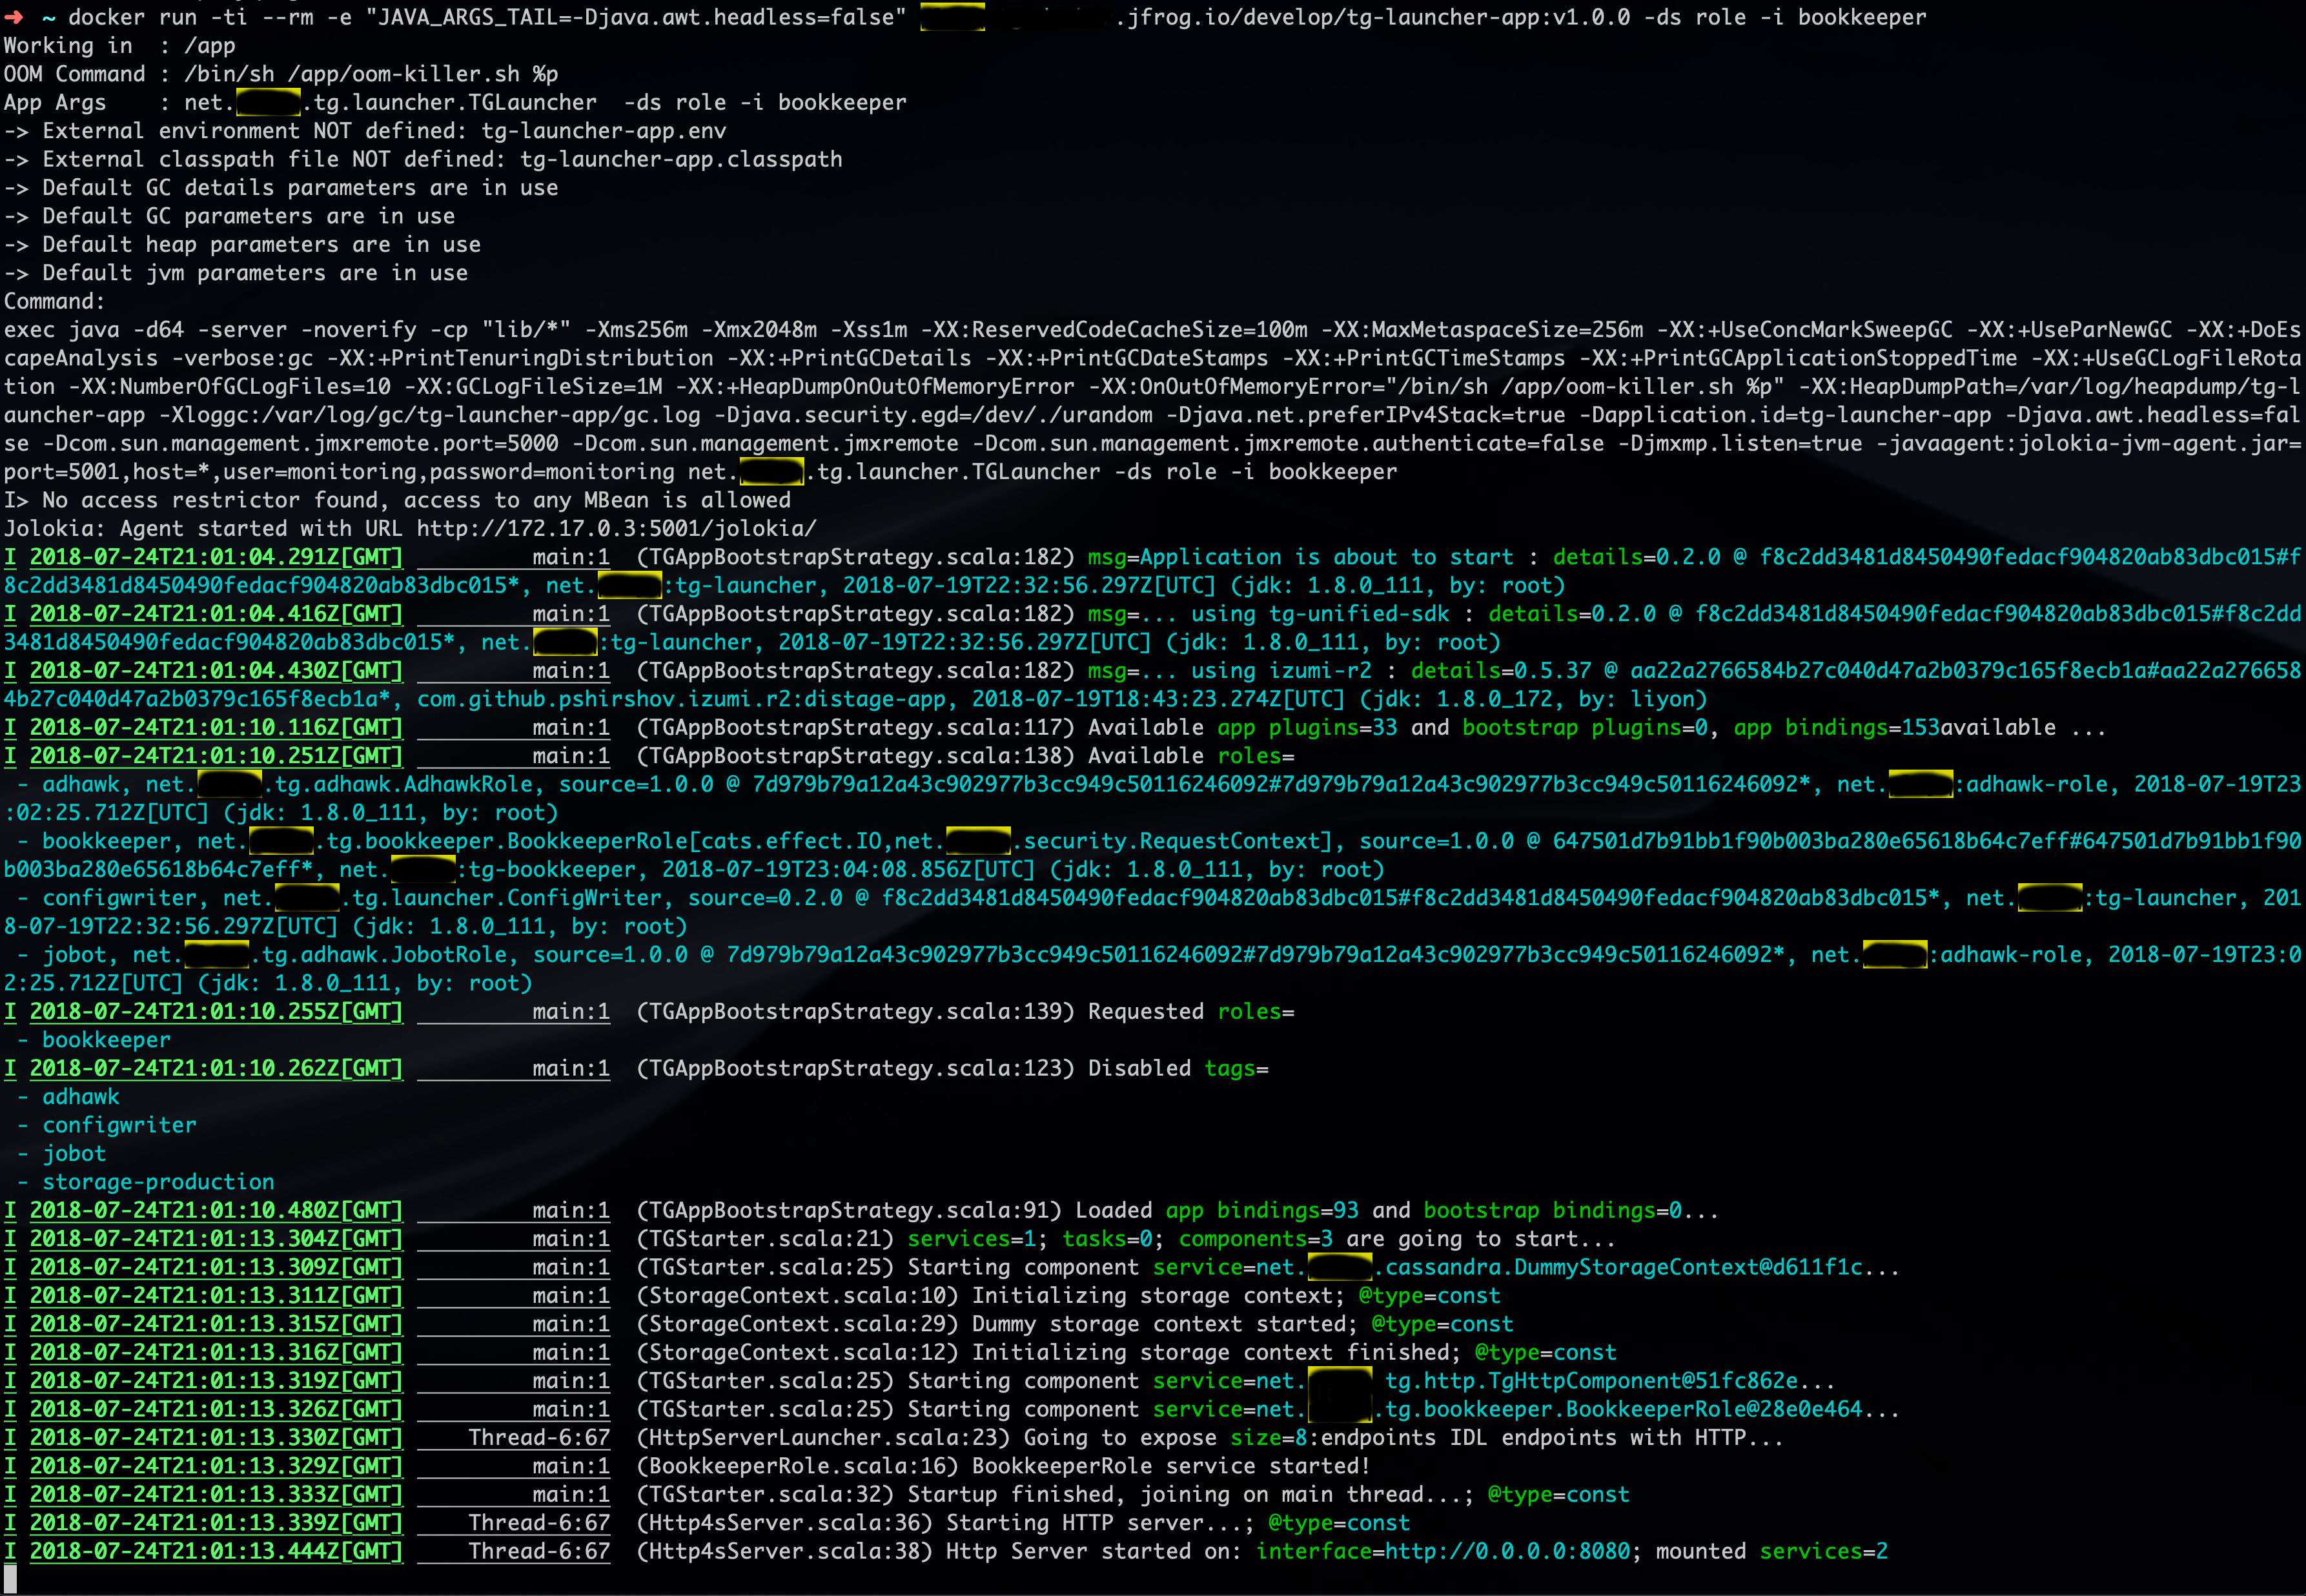
\includegraphics[width=\textwidth]{media/roles-example.png}
\end{figure}
\end{frame}

\begin{frame}
\frametitle{Status and things to do}
Distage is:
\begin{itemize}
\item ready to use,
\item in real production for 4 months.
\end{itemize}
\vspace{0.3cm}
Our plans:
\begin{itemize}
\item Make Roles opensource. ASAP,
\item Implement a Testkit,
\item Support optional isolated classloaders (in foreseeable future),
\item Check our GitHub: https://github.com/pshirshov/izumi-r2.
\end{itemize}
\end{frame}

\begin{frame}
\frametitle{DIStage is just a part of our stack}
We have a vision backed by our tools:
\begin{itemize}
\item Idealingua: transport and codec agnostic gRPC alternative with rich modeling language,
\item LogStage: zero-cost logging framework,
\item \textit{Fusional Programming and Design} guidelines. We love both FP and OOP,
\item \textit{Continous Delivery} guidelines for Role-based process, 
\item \textit{Percept-Plan-Execute} Generative Programming approach, abstract machine and computational model.
Addresses Project Planning (see Operations Research). Examples: orchestration, build systems.
\end{itemize}

Altogether these things already allowed us to significantly reduce development costs and
delivery time for our client.\newline

More slides to follow.
\end{frame}

\begin{frame}
    \frametitle{Thank you for your attention}

    \begin{center}
      https://izumi.7mind.io/

      We're looking for clients, contributors, adopters and colleagues ;)
    \end{center}

    About the author:
    \begin{itemize}
        \item coding for 18 years, 10 years of hands-on commercial engineering experience,
        \item has been leading a cluster orchestration team in Yandex, ``the Russian Google'',
        \item implemented ``\textit{Interstellar Spaceship}'' -- an orchestration solution to manage 50K+ physical machines across 6 datacenters,
        \item Owns an Irish R\&D company, https://7mind.io,
        \item Contacts: team@7mind.io,
        \item Github: https://github.com/pshirshov
    \end{itemize}
\end{frame}

\end{document}
